% Where the safeguards sit: a chat model's refusals come from safety training,
% with classifiers added by some hosted services; a biological sequence model
% has no refusal layer, and relies on what was left out of training and on the
% screening of DNA orders. Prompt injection acts on the agent that uses either.
% ---------------------------------------------------------------------------
% style.tex --- shared preamble for every figure in book/figures/tikz/
%
% One style for all figures: Latin Modern, thin black lines, a light grey
% fill, and one accent colour used only to mark what is untrusted or wrong.
% Build with scripts/build_figures.sh; see book/figures/README.md.
% ---------------------------------------------------------------------------
\documentclass[tikz,border=6pt]{standalone}
\usepackage[T1]{fontenc}
\usepackage{lmodern}
\usetikzlibrary{arrows.meta,positioning,shapes.geometric,calc,fit,backgrounds}

\hyphenpenalty=10000   % short lines in boxes: ragged, never hyphenated

\definecolor{lightgrey}{gray}{0.92}
\definecolor{accent}{HTML}{9B2D20}

\tikzset{
  every picture/.style={
    line width=0.6pt,
    font=\small,
    >={Stealth[length=5pt,width=4pt]},
    node distance=14pt and 24pt,
  },
  % shapes
  box/.style={draw, rectangle, inner xsep=8pt, inner ysep=5pt,
              minimum height=22pt, align=center},
  grey/.style={box, fill=lightgrey},
  rounded/.style={box, rounded corners=9pt},
  decision/.style={draw, diamond, aspect=2.4, inner sep=1.5pt, align=center},
  group/.style={draw, dashed, rounded corners=5pt, inner sep=7pt},
  % text
  tag/.style={font=\footnotesize, align=center, inner sep=2pt},
  note/.style={font=\footnotesize\itshape, align=center, inner sep=2pt},
  code/.style={font=\small\ttfamily},
  codetag/.style={font=\footnotesize\ttfamily, align=center, inner sep=2pt},
  title/.style={font=\small\scshape, align=center, inner sep=2pt},
  % lines
  arrow/.style={->},
  back/.style={->, dashed},
  thin/.style={line width=0.4pt, gray},
  % the one accent, for what is untrusted, wrong or missing
  bad/.style={accent},
  badbox/.style={box, draw=accent, text=accent},
}

\begin{document}
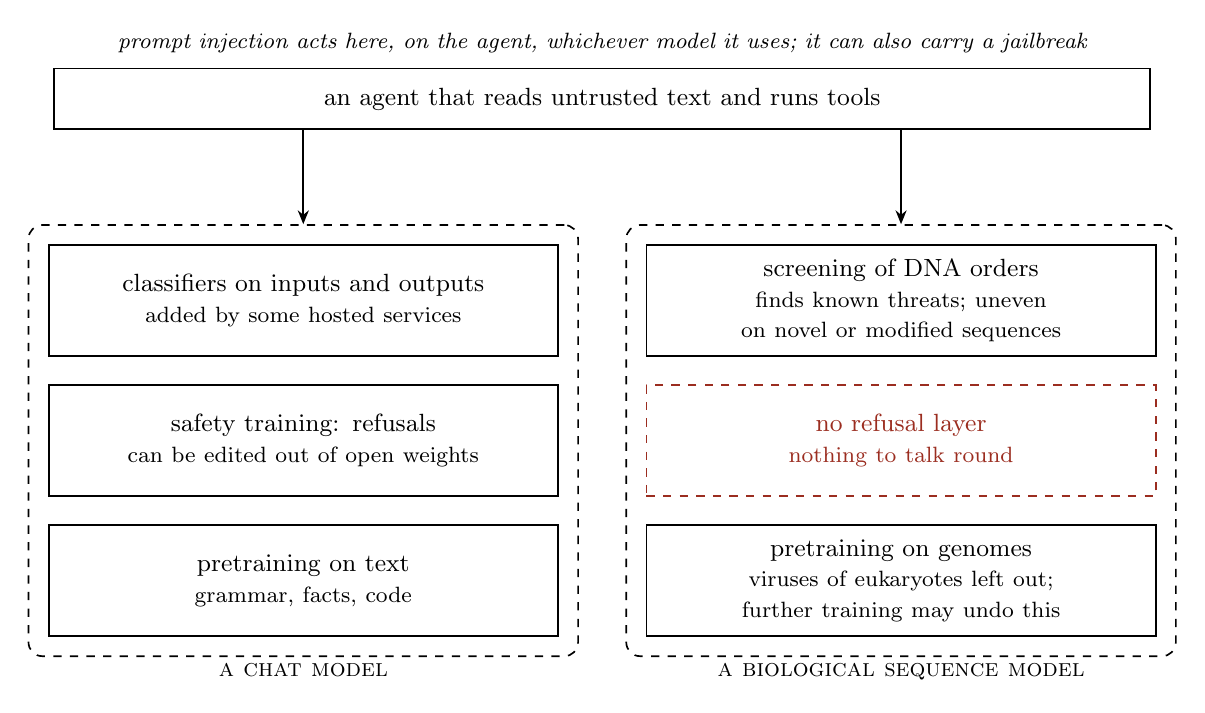
\begin{tikzpicture}[col/.style={box, text width=168pt, minimum height=40pt}]
  % a chat model, bottom to top
  \node[col] (lpre) at (-108pt,0) {pretraining on text\\ \footnotesize grammar, facts, code};
  \node[col, above=10pt of lpre] (lsafe) {safety training: refusals\\ \footnotesize can be edited out of open weights};
  \node[col, above=10pt of lsafe] (lcls) {classifiers on inputs and outputs\\ \footnotesize added by some hosted services};
  \node[group, fit=(lpre) (lcls), label={[title]below:a chat model}] (lgrp) {};
  % a biological sequence model, bottom to top
  \node[col] (rpre) at (108pt,0) {pretraining on genomes\\ \footnotesize viruses of eukaryotes left out; further training may undo this};
  \node[badbox, col, draw=accent, dashed, above=10pt of rpre] (rnone) {no refusal layer\\ \footnotesize nothing to talk round};
  \node[col, above=10pt of rnone] (rscr) {screening of DNA orders\\ \footnotesize finds known threats; uneven on novel or modified sequences};
  \node[group, fit=(rpre) (rscr), label={[title]below:a biological sequence model}] (rgrp) {};
  % the agent that uses either
  \node[box, text width=380pt, above=34pt of $(lgrp.north)!0.5!(rgrp.north)$] (agent)
    {an agent that reads untrusted text and runs tools};
  \node[note, above=3pt of agent, text width=380pt]
    {prompt injection acts here, on the agent, whichever model it uses; it can also carry a jailbreak};
  \draw[->] (agent.south -| lgrp.north) -- (lgrp.north);
  \draw[->] (agent.south -| rgrp.north) -- (rgrp.north);
\end{tikzpicture}
\end{document}
